\documentclass{beamer}
\usepackage{beamerthemeshadow}
\usepackage{tabulary}
\usepackage{xcolor}
\usepackage{mathtools}
\usepackage{amsmath}
\usepackage{graphicx}
\usepackage{lmodern}% http://ctan.org/pkg/lm
\usepackage[mediumspace,mediumqspace,squaren]{SIunits}

\usetheme{Copenhagen}
\usecolortheme{crane}
%\useinnertheme{circles}
\usefonttheme{structurebold}
\usefonttheme[onlymath]{serif}

%\usepackage[english]{babel}
%\usepackage[latin1]{inputenc}
%\usepackage{times}
%%\usepackage[T1]{fontenc}


\setbeamerfont{page number in head/foot}{size=\small}
\setbeamerfont{caption}{size=\tiny}
%\usepackage[textfont={big,it}]{caption}
\setbeamertemplate{footline}[frame number]

\beamersetuncovermixins{\opaqueness<1>{25}}{\opaqueness<2->{15}}
\begin{document}
\title{Smartphones - From vacuum tubes to integrated circuits} 
\author{Nik Dennler}
\date{\today} 

\begin{frame}
\titlepage
\end{frame} 

\begin{frame}\frametitle{Table of Contents}\tableofcontents
\end{frame} 


\section{Historical and current electric circuits and devices} 
\subsection{Analog Circuits}
\begin{frame}\frametitle{Analog Circuits} 
\begin{columns}
\begin{column}{6cm}
\begin{itemize}
\item Threshold of the current or voltage varies continuously over time\pause
\item Constructed from serial and parallel circuits \pause
\item Obeying Kirchhoff's circuit laws: 
\begin{equation*}
 \sum_{k=1}^{n} I_{k} = 0 \text{    ,    } \sum_{k=1}^{n} V_{k} = 0
\end{equation*}

\end{itemize}
%\vspace{3cm} 
\end{column}
\begin{column}{6cm}
\begin{figure}
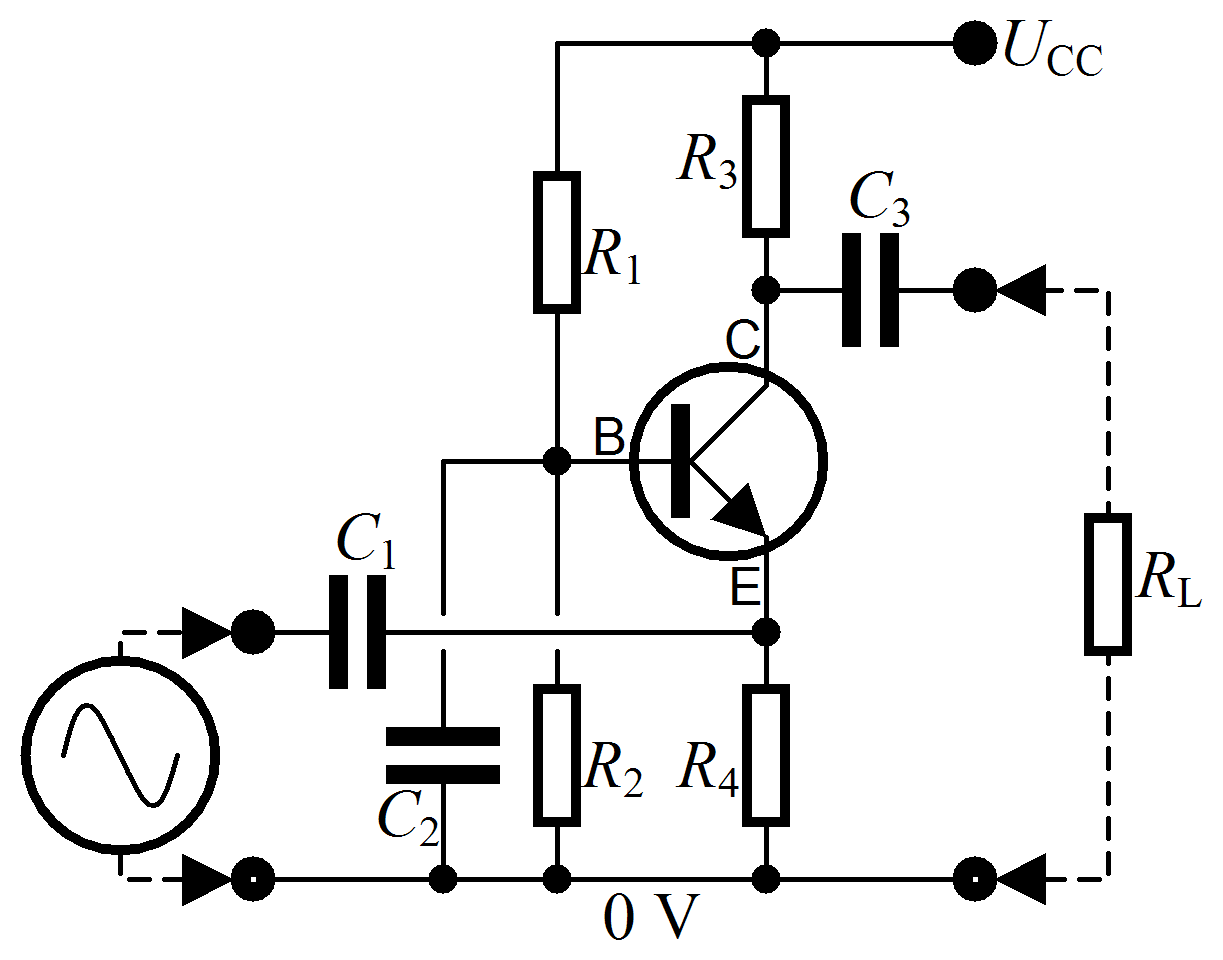
\includegraphics[width=0.8\textwidth]{ampcircuit}
\caption{\url{https://en.wikipedia.org/wiki/Electronic_circuit}}
%\label{fig:ampcircuit}
\end{figure}
%\caption{\url{https://en.wikipedia.org/wiki/Electronic_circuit}}
\end{column}
\end{columns}
\end{frame}

\subsection{Digital Circuits}
\begin{frame}\frametitle{Digital Circuits} 
\begin{itemize}
\item Electric signals take on discrete values to represent logical and numeric values \pause
\item Mostly, binary encoding is used: one voltage represents a binary '$1$' and another voltage the binary '$0$' \pause
\item Binary digits can be used to represent numbers and characters and therefore convey information \pause
\item The binary code was invented by Gottfried Leibniz in 1679
\end{itemize}
\end{frame}

\begin{frame}\frametitle{Binary Representation} 
\begin{columns}
\begin{column}{6cm}
\begin{figure}
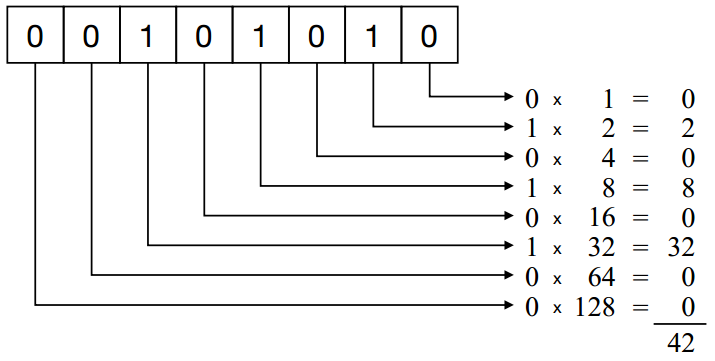
\includegraphics[width=1\textwidth]{binary.png}%
\caption{\url{http://binarynumbersa.blogspot.ch/2012/02/representation-of-binary-numbers.html}}%
%\label{fig:binary}
\end{figure}
%\caption{\url{https://en.wikipedia.org/wiki/Electronic_circuit}}
\end{column}
\begin{column}{6cm}
\begin{figure}
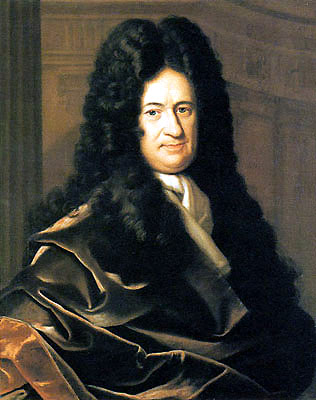
\includegraphics[width=0.5\textwidth]{leibniz}%
\caption{\url{https://en.wikipedia.org/wiki/.../media/File:Gottfried_Wilhelm_von_Leibniz}}%
%\label{fig:binary}
\end{figure}
%\caption{\url{https://en.wikipedia.org/wiki/Electronic_circuit}}
\end{column}
\end{columns}
\end{frame}

\begin{frame}\frametitle{Bool Algebra and logical circuits}
\begin{columns}
\begin{column}{6cm}
\begin{itemize}
\item<1-> Conjunction: $a\land b$ is $True$, if $a$ is $True$ and $b$ is $True$.\\
\pause
\item<2-> Disjunction: $a\lor b$  is $True$, if $a$ is $True$ or $b$ is $True$ or $a\wedge b$ is $True$.\\
\pause
\item<3-> Negation:  $\neg a$ is $True$, if $a$ is $False$. 
\pause
\item<4-> Associative, Commutative and Distributive
\pause
\item<5-> Neutral-, Inverse- and a Zero element
\end{itemize}
%\vspace{3cm} 
\end{column}
\begin{column}{6cm}
\only<3->{
\begin{table}[H]
\centering
\begin{tabular}{c|c|c|c|c}
\textbf{$a$} & \textbf{$b$} & \textbf{$a\land b$} & \textbf{$a\lor b$} & \textbf{$\neg a$} \\ \hline
0          & 0          & 0            & 0            & 1           \\
1          & 0          & 0            & 1            & 0           \\
0          & 1          & 0            & 1            & 1           \\
1          & 1          & 1            & 1            & 0          
\end{tabular}
\caption{Truth-table}
%\label{tab:truth}
\end{table}}
%\caption{\url{https://en.wikipedia.org/wiki/Electronic_circuit}}
\end{column}
\end{columns}
\end{frame}

\begin{frame}\frametitle{Vacuum tubes} 
\begin{columns}
\begin{column}{7cm}
\begin{itemize}
\item<1-> Controls electric current between electrodes in an evacuated container
\item<2-> 1880: Thermionic emission (Edinson-Richardson-Effect)
\begin{equation*} 
%\label{eq:J}
J=A\cdot T^2 \cdot e^{-\frac{W_e}{k \cdot T}}
\end{equation*}
\item<3-> 1904: Diode (John Fleming)
\item<4-> 1907: Triode (Lee de Forrest) 
\end{itemize}
\end{column}
\begin{column}{4cm}
\begin{overprint}
\only<3>{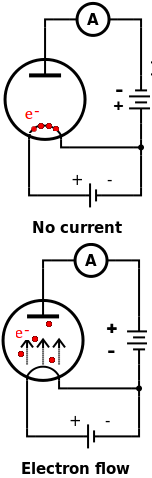
\includegraphics[width=0.47\textwidth]{edisoneffect}}%
\only<4->{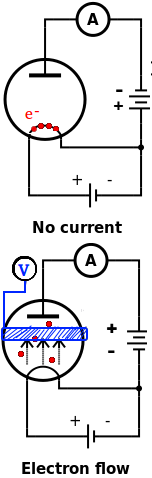
\includegraphics[width=0.47\textwidth]{edisoneffect_triode}}%
\end{overprint}
%\caption{\url{https://en.wikipedia.org/wiki/Electronic_circuit}}
\end{column}
\end{columns}
\end{frame}

\begin{frame}\frametitle{Vacuum tubes} 
\begin{columns}
\begin{column}{6cm}
\begin{figure}[H]
\centering
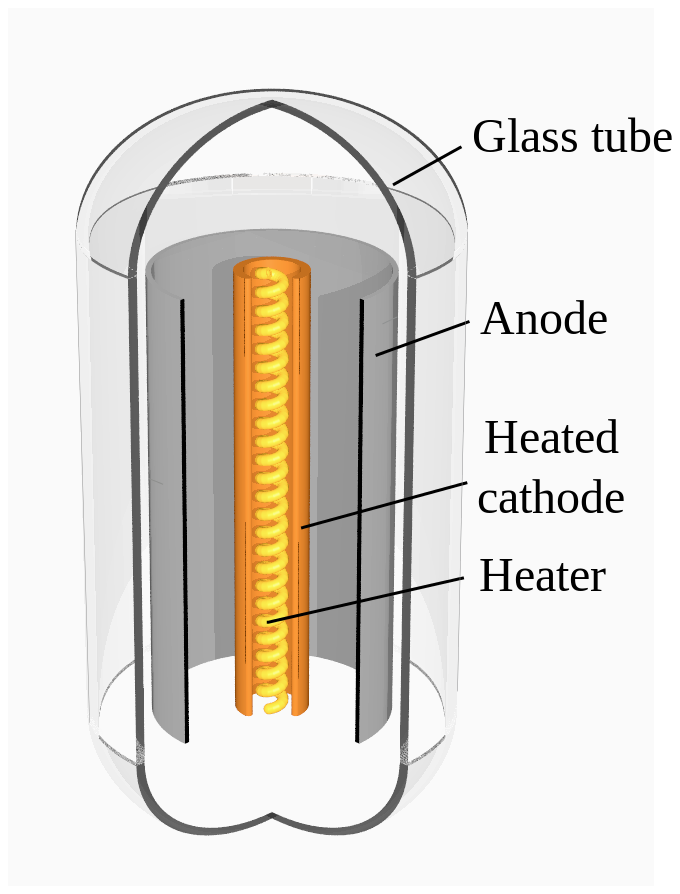
\includegraphics[width=0.6\textwidth]{diode}%
\caption{\url{https://en.wikipedia.org/wiki/.../media/File:Diode.svg}}%
%\label{fig:diode}
\end{figure}
\end{column}
\begin{column}{6cm}
\begin{figure}[H]
\centering
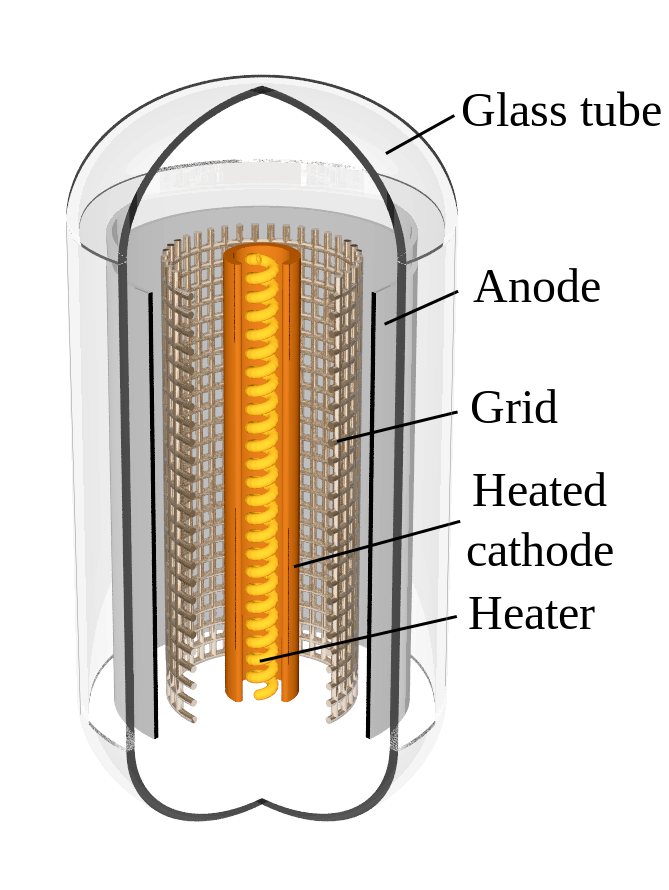
\includegraphics[width=0.6\textwidth]{triode}%
\caption{\url{https://en.wikipedia.org/wiki/.../media/File:Triode.svg}}%
%\label{fig:triode}
\end{figure}
%\caption{\url{https://en.wikipedia.org/wiki/Electronic_circuit}}
\end{column}
\end{columns}
\end{frame}

\begin{frame}\frametitle{ENIAC}
\begin{figure}[H]
\centering
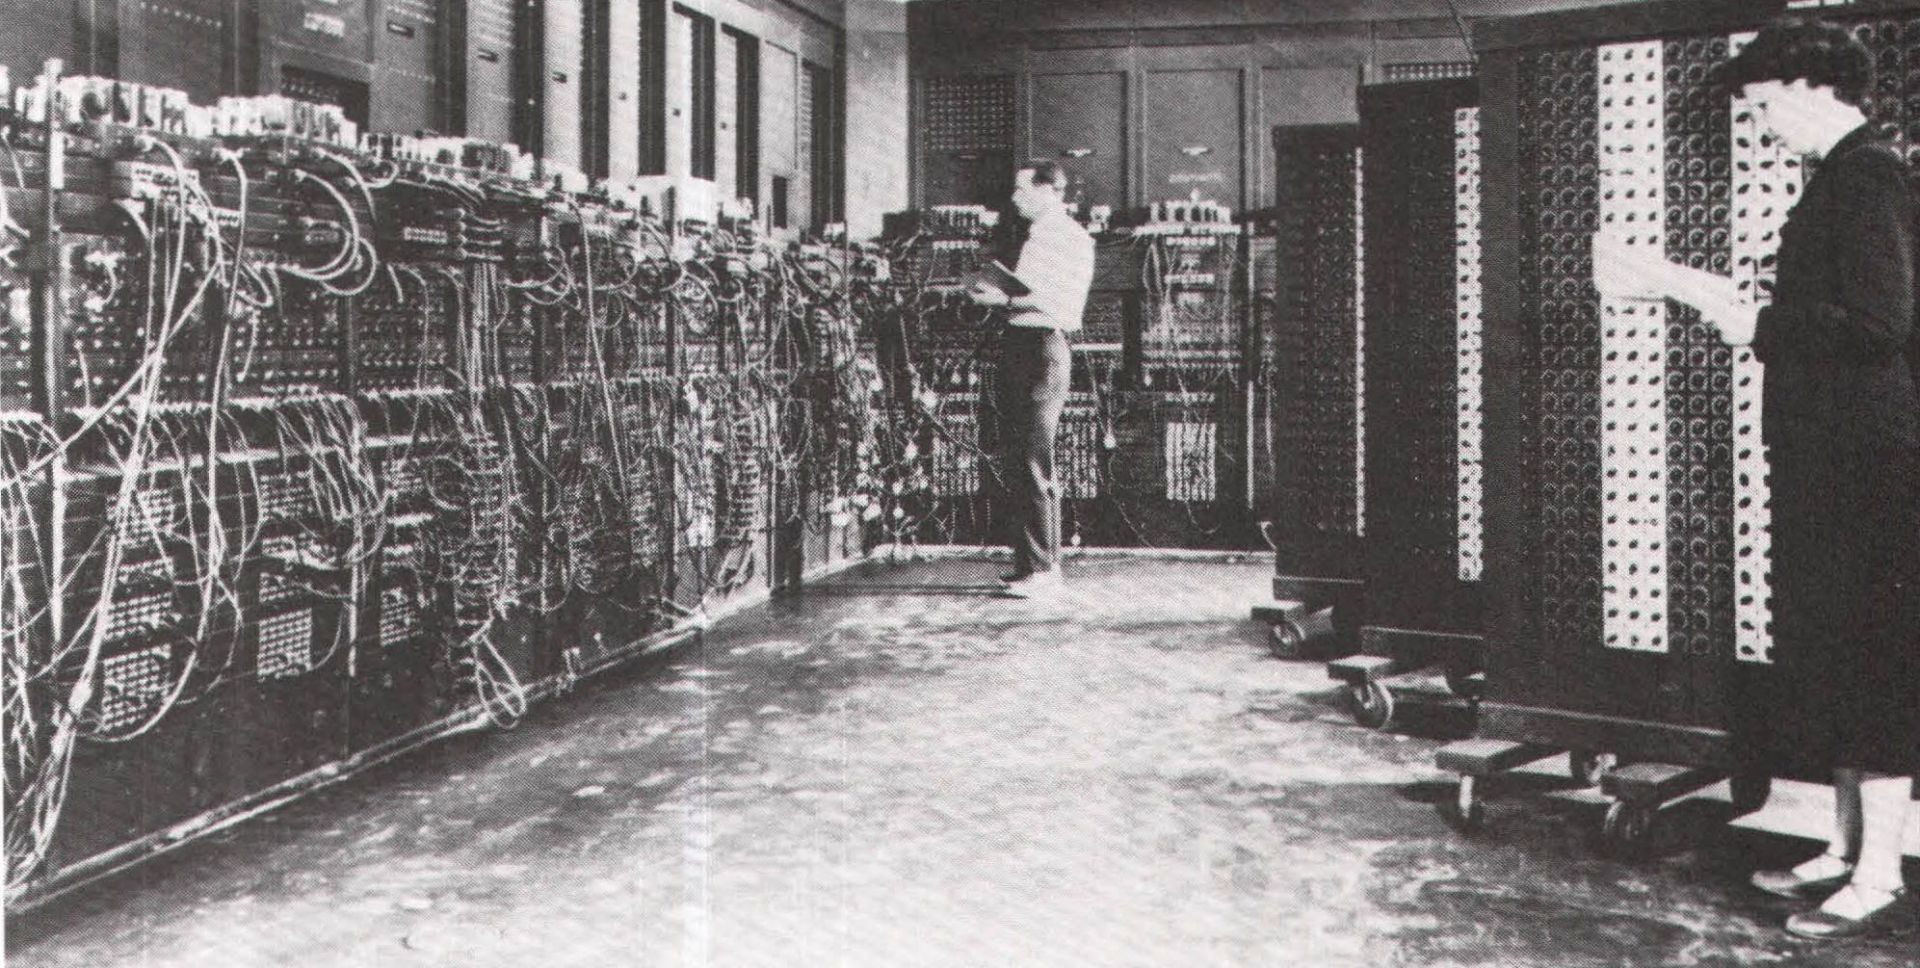
\includegraphics[width=0.9\textwidth]{eniac}%
\caption{\url{http://www.cs.kent.edu}}%
%\label{fig:eniac}
\end{figure}
\end{frame}


\begin{frame}\frametitle{Transistors} 
\begin{columns}
\begin{column}{6cm}
\begin{itemize}
\item Triode based on semiconductor properties
\pause
\item Invented in 1934 by Oskar Heil
\pause
\item Can be used as On/Off switch or amplifier
\pause
\item Transformed the way we live!
\end{itemize}
%\vspace{3cm} 
\end{column}
\begin{column}{6cm}
\begin{figure}[H]
\centering
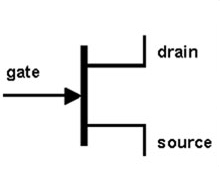
\includegraphics[width=0.65\textwidth]{transistor}%
\caption{\url{Sze, Semiconductor Devices}}%
%\label{fig:transistor}
\end{figure}
%\caption{\url{https://en.wikipedia.org/wiki/Electronic_circuit}}
\end{column}
\end{columns}
\end{frame}



\begin{frame}\frametitle{Logic gates \& Integrated Circuits} 
\begin{columns}
\begin{column}{5cm}
\begin{itemize}
\item<1-> Multiple Transistors can form (Bool-) logic gates 
\item<2-> Logic gates printed on silicon wafer to form an integrated circuit
\end{itemize}
\end{column}
\begin{column}{6cm}
\begin{overprint}
\only<1>{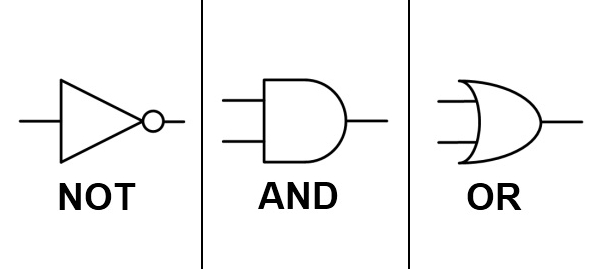
\includegraphics[width=0.94\textwidth]{logicg}}%
\only<2>{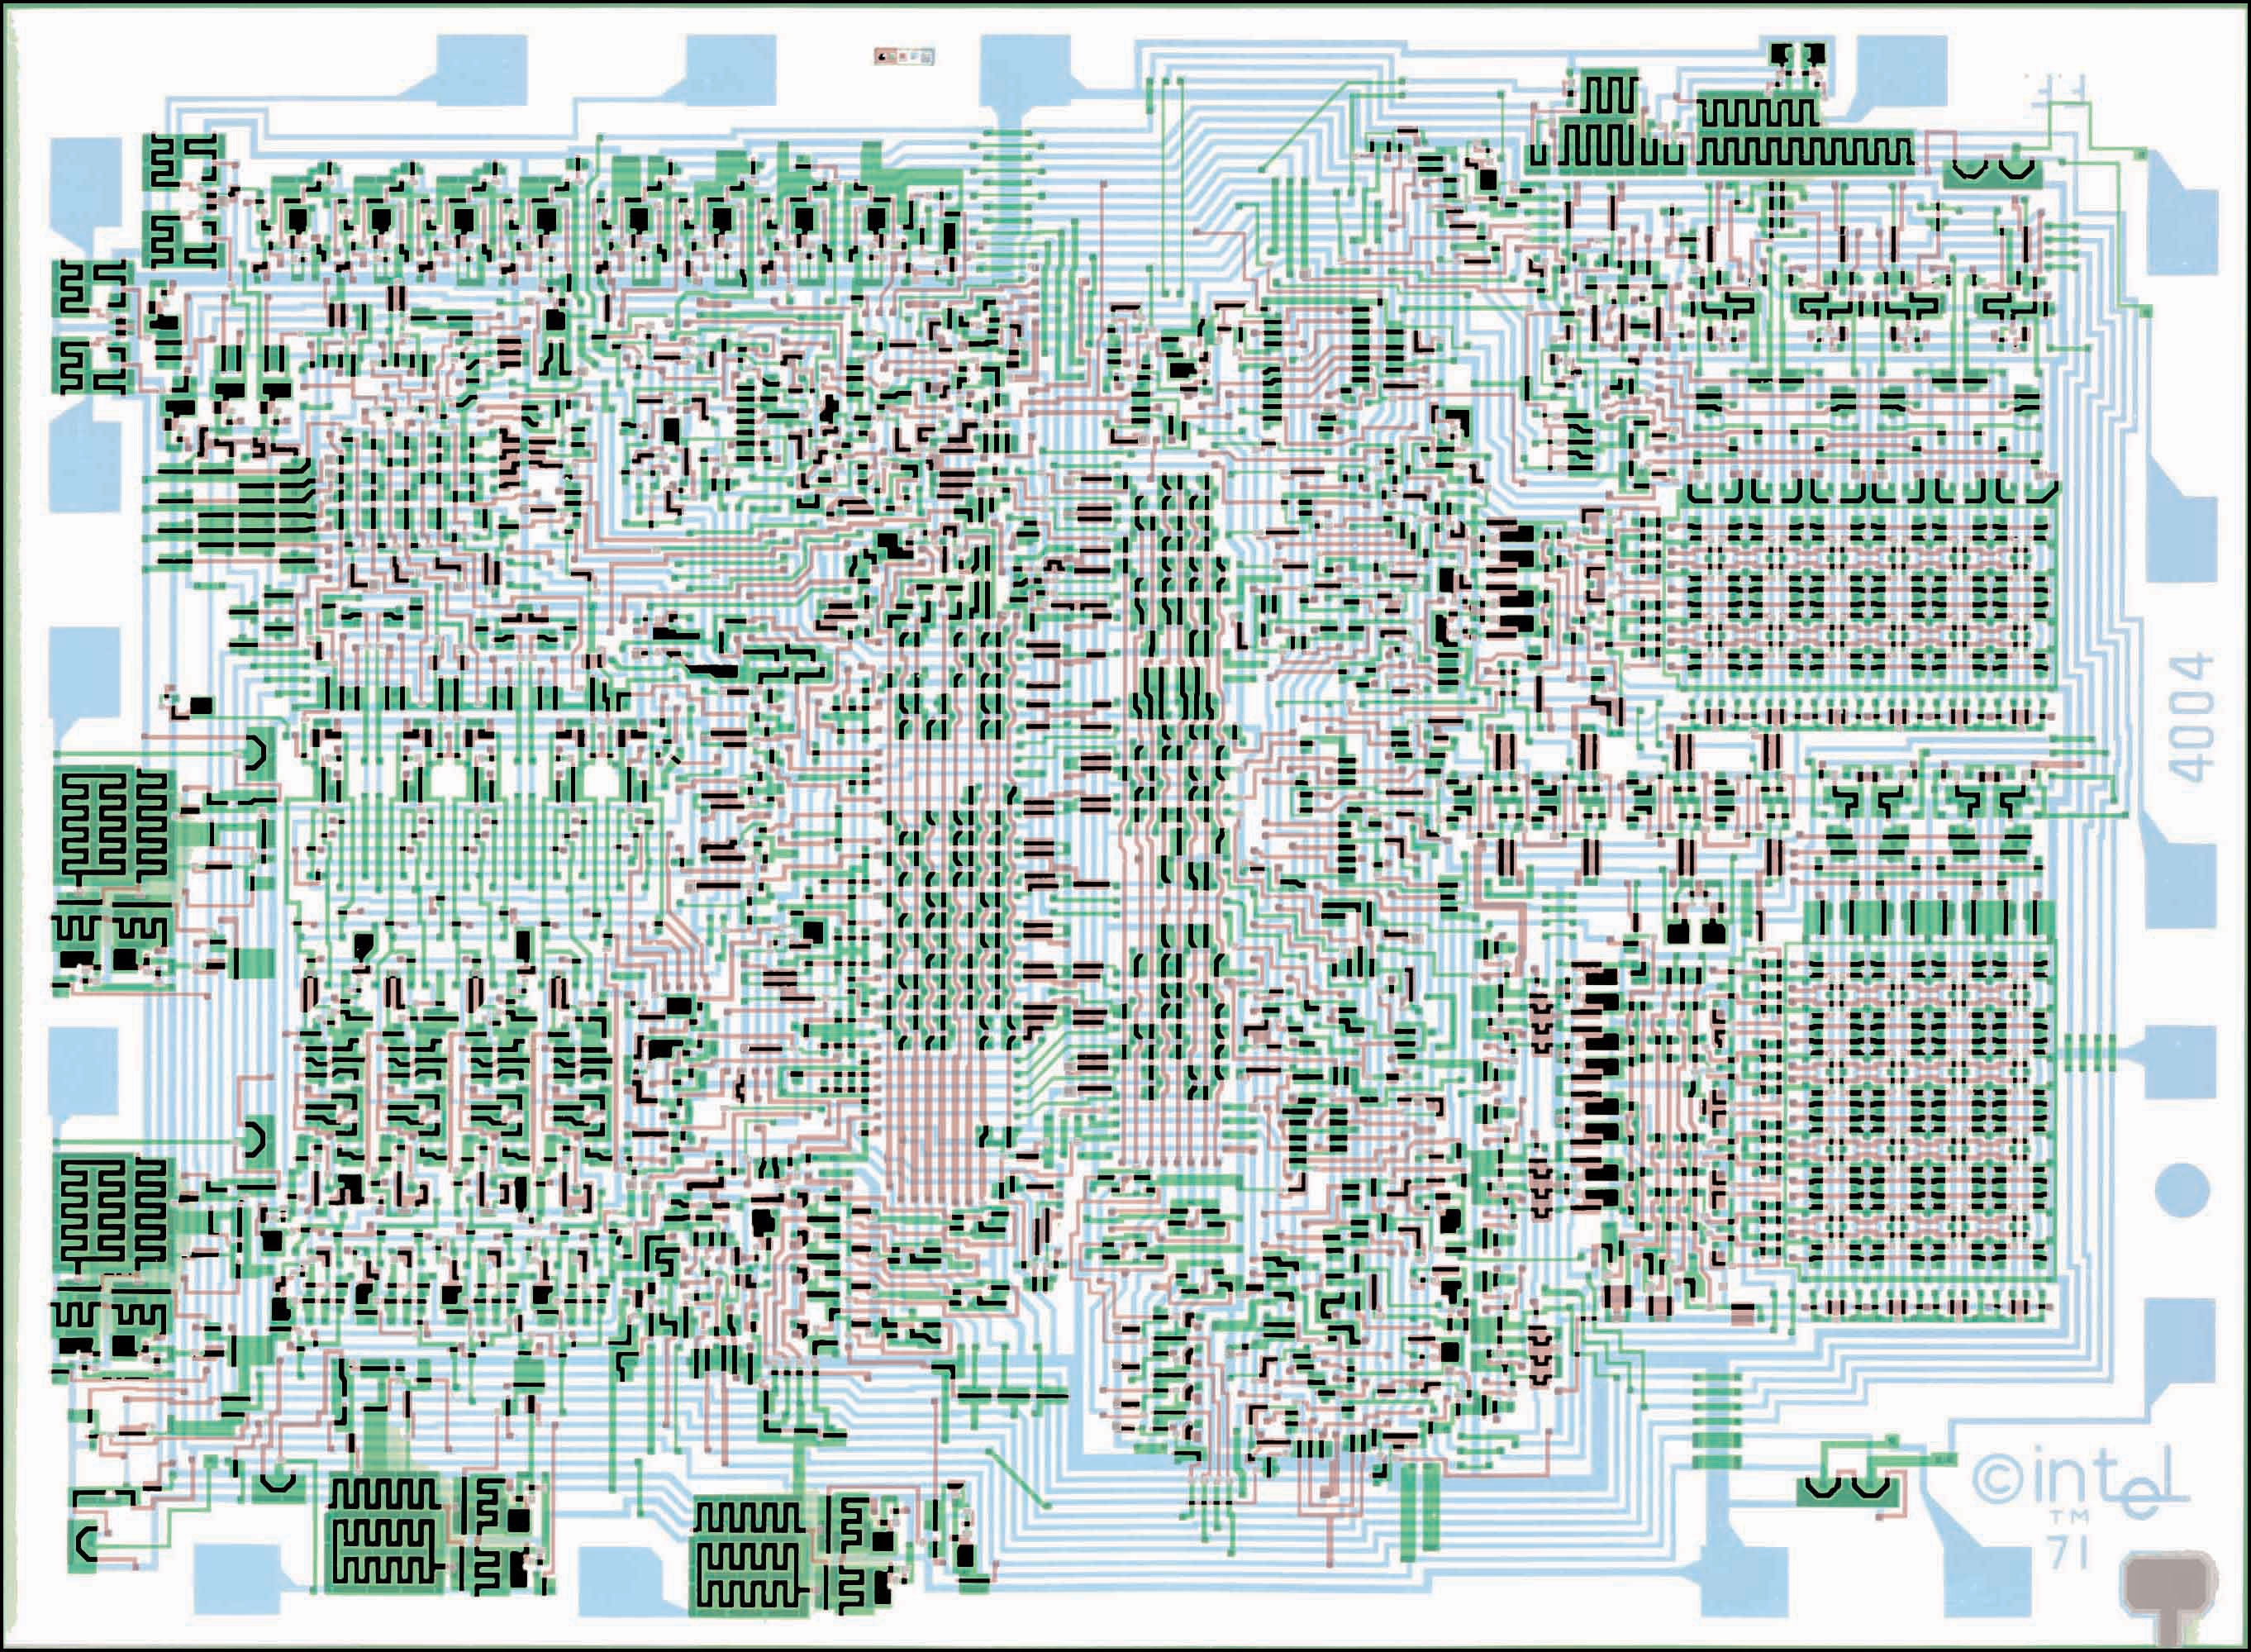
\includegraphics[width=1\textwidth]{4004}}
\only<1>{\mbox{\structure{\tiny{Figure:}}\tiny{ \url{http://www.mibb-design.com}}}}
\only<2>{\mbox{\structure{\tiny{Figure:}}\tiny{ \url{http://www.4004.com}}}}

\end{overprint}
\end{column}
\end{columns}
\end{frame}


\section{How does a transistor work?} 
\subsection{Semiconductors}
\begin{frame}\frametitle{Semiconductors} 
\begin{columns}
\begin{column}{6cm}
\begin{itemize}
\item<1-> Electric conductivity between conductor and insulator
\pause
\item<2-> Electrons follow Fermi-dirac distribution:
\begin{equation*} 
%\label{eq:Fermi}
f(E) = \frac{1}{1 + e^{\frac{E - \epsilon_F}{k \cdot T} } }
\end{equation*}
\pause
\item<3-> All electrons combined form energy bands
\pause
\item<4-> Band gap size between conductor and insulator
\end{itemize}
%\vspace{3cm} 
\end{column}
\begin{column}{6cm}
%\begin{overprint}
\begin{figure}[H]
\centering
\includegraphics<2>[width=0.55\textwidth]{fermi}
%\caption{\url{U. Tietze, Halbleiter-Schaltungstechnik}}%
%\label{fig:fermi}
%\end{figure}}

%\begin{figure}[H]
%\centering
\includegraphics<3->[width=0.85\textwidth]{energyband}\caption{{U. Straumann, Elektronik fur Physiker}}
%\label{fig:energyband}
\end{figure}
%\end{overprint}
\end{column}
\end{columns}
\end{frame}

\begin{frame}\frametitle{Doping} 
\begin{columns}
\begin{column}{6cm}
\begin{itemize}
\item<1-> Infusing impurities into material increases number of free charges
\pause
\item<2-> \textit{n-doping}: infusing valence+1 atom, creates additional electron state
\pause
\item<3-> \textit{p-doping}: infusing valence-1 atom, creates additional hole state
\end{itemize}
%\vspace{3cm} 
\end{column}
\begin{column}{5cm}
%\begin{overprint}
\begin{figure}[H]
\centering
\includegraphics<1->[width=1\textwidth]{donator}
%\caption{\url{U. Tietze, Halbleiter-Schaltungstechnik}}%
%\label{fig:donator}
%\end{figure}}

%\begin{figure}[H]
%\centering
\includegraphics<3->[width=1\textwidth]{acceptor}\caption{{Ch. Kittel, Solid State Physics}}
%\label{fig:acceptor}
\end{figure}
%\end{overprint}
\end{column}
\end{columns}
\end{frame}

\begin{frame}\frametitle{p-n junction} 
\begin{columns}
\begin{column}{6.2cm}
\begin{itemize}
\item<1-> Diffusion moves excess charges between p- and n-area. $\rightarrow$ electric field

\item<2-> Equilibrium between diffusion and electric potential: \textit{depletion zone}

\item<3-> \textit{Forward-bias}: positive current on p-area decreases the depletion zone, allows electrons to flow.

\item<4-> \textit{Reverse-bias}: negative current on p-area increases the depletion zone, junction behaves as insulator.
\end{itemize}
%\vspace{3cm} 
\end{column}
\begin{column}{4.8cm}
%\begin{overprint}
\begin{figure}[H]

\includegraphics<1->[width=1.1\textwidth]{pn_junction}
\caption{\url{https://en.wikipedia.org/.../File:Pn-junction-equilibrium-graphs.png}}%
%\label{fig:pn_junction}
\end{figure}
%\end{overprint}
\end{column}
\end{columns}
\end{frame}


\subsection{Transistors}
\begin{frame}\frametitle{Bipolar Junction Transistor (BJT)} 
\begin{columns}
\begin{column}{6cm}
\begin{itemize}
\item<1-> Combination of two junction diodes (\textit{n-p-n} or \textit{p-n-p}) \newline

\item<2-> Emitter, Base, Collector \newline

\item<3-> Emitter-Collector-current is controlled by current on base. \newline

\item<4-> EB in forward-bias, BE in reverse-bias

\end{itemize}
%\vspace{3cm} 
\end{column}
\begin{column}{5cm}
%\begin{overprint}
\begin{figure}[H]
\centering
\includegraphics<1->[width=1.1\textwidth]{npn}
\caption{\url{http://www.electronics-tutorials.ws}}%
%\label{fig:npn}
\end{figure}
%\end{overprint}
\end{column}
\end{columns}
\end{frame}

\begin{frame}\frametitle{Field Effect Transistor (FET)} 
\begin{columns}
\begin{column}{6cm}
\begin{itemize}
\item<1-> Conductivity bases only on electron or hole states (\textit{n-channel} or \textit{p-channel}) \newline

\item<2-> Source, Channel, Gate, Drain \newline

\item<3-> Source-drain-current is controlled by voltage on gate \newline

\end{itemize}
%\vspace{3cm} 
\end{column}
\begin{column}{5cm}
%\begin{overprint}
\begin{figure}[H]
\centering
\includegraphics<1->[width=0.9\textwidth]{jfet_closed}
%\caption{\url{U. Tietze, Halbleiter-Schaltungstechnik}}%
%\label{fig:jfet_closed}
%\end{figure}}

%\begin{figure}[H]
%\centering
\includegraphics<1->[width=0.9\textwidth]{jfet_open}\caption{\url{http://www.electronics-tutorials.ws}}
%\label{fig:jfet_open}
\end{figure}
%\end{overprint}
\end{column}
\end{columns}
\end{frame}

\begin{frame}\frametitle{Field Effect Transistor (FET)} 
\begin{columns}
\begin{column}{6cm}
\begin{itemize}
\item<1-> \textit{Cut-Off Region}: $V_{GS}=0$ $\rightarrow$ no DS-current \newline(Off-Region)

\item<2-> \textit{Ohmic Region}: $V_{GS}>0$ and $V_{DS}$ small $\rightarrow$ current controlled by $V_{DS}$

\item<3-> \textit{Saturation Region}: $V_{GS}>0$ and $V_{DS}$ large $\rightarrow$ DS-current controlled by drain voltage  \newline(On-Region)

\item<4-> \textit{Breakdown Region}: $V_{DS}$ very large $\rightarrow$ maximum current

\end{itemize}
%\vspace{3cm} 
\end{column}
\begin{column}{5cm}
%\begin{overprint}
\begin{figure}[H]
\centering
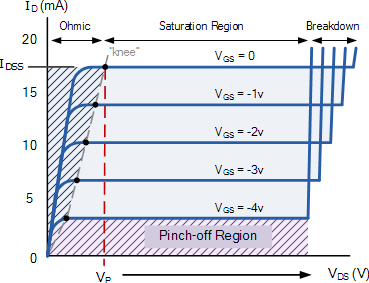
\includegraphics[width=0.9\textwidth]{kenn_jfet}
\caption{\url{http://www.electronics-tutorials.ws}}%
%\label{fig:kenn_jfet}
\end{figure}
%\end{overprint}
\end{column}
\end{columns}
\end{frame}

\begin{frame}\frametitle{MOSFET} 
\begin{columns}
\begin{column}{6cm}
\begin{itemize}
\item<1-> JFET architecture, but small $SiO_2$ layer between gate and channel 

\item<2-> Insulating layer raises the input resistance of the MOSFET and prevents any channel-gate-current

\end{itemize}
%\vspace{3cm} 
\end{column}
\begin{column}{5cm}
%\begin{overprint}
\begin{figure}[H]
\centering
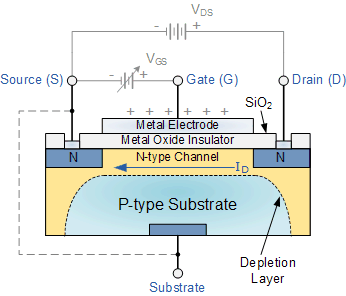
\includegraphics[width=0.9\textwidth]{mosfet}
\caption{\url{http://www.electronics-tutorials.ws}}%
%\label{fig:mosfet}
\end{figure}
%\end{overprint}
\end{column}
\end{columns}
\end{frame}

\begin{frame}\frametitle{MOSFET} 
\begin{columns}
\begin{column}{6cm}
\begin{itemize}
\item Electrons in conducting band, holes in valence band 
\item In Off-state can charge carriers not pass big potential wall
\item In On-state the potential wall is lowered and charges can pass
\end{itemize}
\end{column}
\begin{column}{5cm}
%\begin{overprint}
\includegraphics<1>[width=0.9\textwidth]{MOSFETvs}
\end{column}
\end{columns}
\end{frame}

\begin{frame}\frametitle{Differences, advantages and disadvantages of BJTs and MOSFETs} %%make table! appearing, with colors!
\begin{tabulary}{\linewidth}{L | L}
\textbf{BJT} & \textbf{MOSFET} \\
\hline
emitter, collector, base & gate, source, channel, drain  \\
\hline
electron and hole state conduction & either electron or hole state conduction \\
\hline
controlled by current & controlled by voltage  \\
\hline
\textcolor{green}{less complex} &      \\
\hline
    &  \textcolor{red}{vulnerable to electrostatic damage during installation} \\
\end{tabulary}
\end{frame}

\begin{frame}\frametitle{Differences, advantages and disadvantages of BJTs and MOSFETs} %%make table! appearing, with colors!
\begin{tabulary}{\linewidth}{L | L}
\textbf{BJT} & \textbf{MOSFET} \\
\hline
  $\ \ \ \ \ \ \ \ \ \ \ \ \ \ \ \ \ \ \ \ \ \ $ & \textcolor{green}{much less leak current}  \\
\hline
   & \textcolor{green}{no additional power draw after the gate is opened or closed} \\
\hline
   & \textcolor{green}{more resistent againt radiation}   \\
\hline
\end{tabulary}
$\ $
\newline \newline
$\rightarrow$ Nowadays, if in digital and analog circuits, MOSFETs are more commonly used than BJTs.
\end{frame}

\section{Future Solutions and Applications} 
\begin{frame}\frametitle{What do we demand of a transistor?} 
\begin{itemize}
\pause
\item Speed: high electron current from source to drain
\pause
\item Reliability: high On/Off current ratio
\pause
\item Low power consumption: low leak current through low subthreshold swing (the voltage required to raise/lower the potential wall by a factor of 10)
 \begin{equation*}
 S_{s-th}=\ln{(10)} \cdot \frac{k_b\cdot T}{e}\cdot(1+\frac{C_D}{C_{ox}}) \pause \geq 60mV/dec
 %\label{eq:subthresholdswing}
 \end{equation*}
\pause
\item Size: As small as possible!
\end{itemize} 
\end{frame}

\subsection{UTB-SOI and FINFET}
\begin{frame}\frametitle{UTB-SOI and FINFET} 
\begin{itemize}
 \item How can the leak current be reduced and the transistor be made smaller?\pause
 
 \item Let's thin the channel! The source will be closer to the gate, which diverts the field lines away from the source\pause
 
 \item Two main approaches: UTB-SOI and FinFET
\end{itemize}
\end{frame}


\begin{frame}\frametitle{Ultrathin Body Silicon on Insulator (UTB-SOI)} 
\begin{columns}
\begin{column}{5cm}
\begin{itemize}
\item<1-> Thin layer of buried oxide on top of base silicon

\item<2-> Very thin channel


\end{itemize}
%\vspace{3cm} 
\end{column}
\begin{column}{7cm}
\begin{center}
\begin{overprint}

\only<1-2>{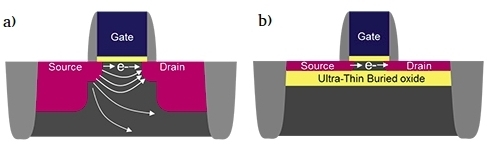
\includegraphics[width=0.8\textwidth]{UTBSOI}}
\only<3>{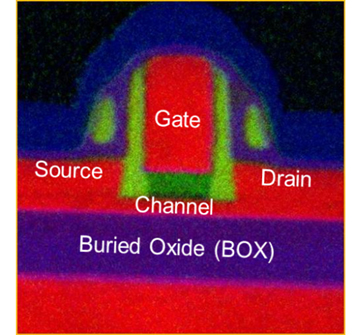
\includegraphics[width=0.4\textwidth]{UTBSOIem}}

\only<1-2>{\mbox{\structure{\tiny{Figure:}}\tiny{ \url{http://www.st.com/.../FD-SOI/learn-more-about-fd-soi.html}}}}
\only<3>{\mbox{\structure{\tiny{Figure:}}\tiny{ \url{http://www.st.com/.../FD-SOI/learn-more-about-fd-soi.html}}}}

\end{overprint}
\end{center}
\end{column}
\end{columns}
\end{frame}

\begin{frame}\frametitle{From 2D to 3D: FinFET} 
\begin{columns}
\begin{column}{5.8cm}
\begin{itemize}
\item<1-> 3D architecture brings the gate closer to the drain

\item<2-> Conducting channel that rises above insulator level, creating a fin-shaped gate electrode

\item<3-> Allows multiple gates on the same device

\item<4-> More drive current per area than 2D architecture \newline $\rightarrow$ faster and less power hungry

\end{itemize}
%\vspace{3cm} 
\end{column}
\begin{column}{6cm}
\begin{center}
\begin{overprint}

\only<1-4>{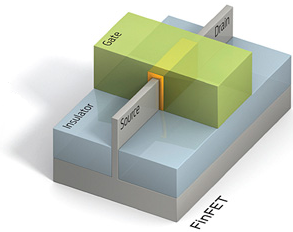
\includegraphics[width=0.7\textwidth]{FinFET}}

\only<1-4>{\mbox{\structure{\tiny{Figure:}}\tiny{ \url{http://www.electronics-tutorials.ws}}}}

\end{overprint}
\end{center}
\end{column}
\end{columns}
\end{frame}


\subsection{Moore's Law}
\begin{frame}\frametitle{Moore's Law}
\begin{columns}
\begin{column}{5cm}
\begin{itemize}
\item<1-> Goal: making the smallest transistor while staying in the cost optimum

\item<2-> \textit{Moore's Law} (1965): The transistor count on an integrated circuit will double every two years

\item<3-> \textit{Intel 4004} (1971): 2300 transistors, $\unit{10}{\micro\meter}$ each 

\item<3-> \textit{Apple A10} (2016): 3'300'000'000 transistors, $\unit{16}{\nano\meter}$ each

\end{itemize}
%\vspace{3cm} 
\end{column}
\begin{column}{7.4cm}
\begin{center}
\begin{overprint}

\only<1>{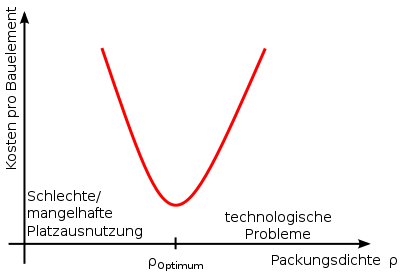
\includegraphics[width=0.5\textwidth]{moore_optimum}}
\only<2-3>{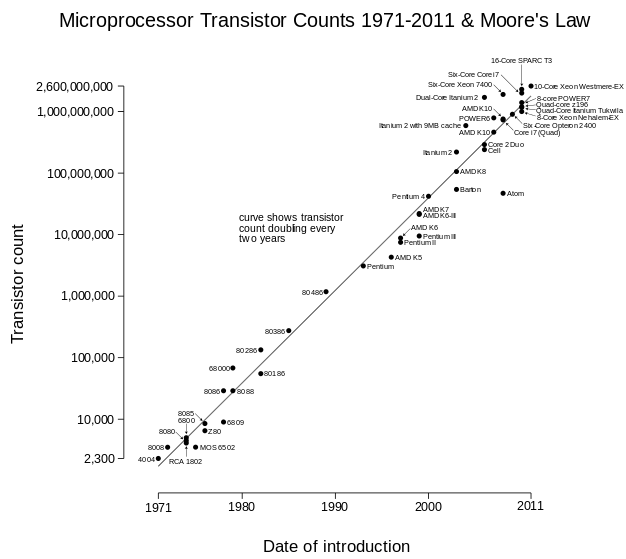
\includegraphics[width=0.82\textwidth]{moore}}

\only<1>{\mbox{\structure{\tiny{Figure:}}\tiny{ \url{https://en.wikipedia.org/wiki/Moores_Law}}}}
\only<2-3>{\mbox{\structure{\tiny{Figure:}}\tiny{ \url{https://en.wikipedia.org/wiki/Moores_Law}}}}

\end{overprint}
\end{center}
\end{column}
\end{columns}
\end{frame}


\subsection{Where does this end?}
\begin{frame}\frametitle{Where does it end?} 
\begin{itemize}
 \item Transistor size gets closer to atomic scale, therefore quantum mechanical phenomenas have to be considered\pause
 \item The tunneling current between channel and gate results in power and information loss\pause
 \item \textit{Intel} estimates, that the miniaturisation of traditional MOSFETs will end in 2020 with a size of $\unit{5}{\nano\meter}$, limited by a \underline{$\unit{1}{\nano\meter}$} gate
\end{itemize}

\end{frame}

\begin{frame}\frametitle{Tunneling probability approximation (WKB)}
\begin{overprint}
\onslide<1>
\begin{itemize}
\item Time independent Schroedinger equation
\begin{equation*}
-\frac{\hbar}{2m^{*}}\frac{d^2\Psi}{dx^2} + (V(x)-E)\Psi = 0,
\end{equation*}
has general solution $\Psi(x)=A e^{kx}+B e^{-kx}$
\item Assume potential is space-independent between $x$ and $x+dx$:
\begin{equation*}
\Psi_{\rightarrow}(x+dx) = \Psi(x)  exp(-k\ dx) \text{,  where  } k=\frac{\sqrt{2m^*[V(x)-E]}}{\hbar}
\end{equation*}
\item Plug in and get WKB approximation integral:
\begin{equation*}
\Psi(L) = \Psi(0) exp(-\int_{0}^{L} \frac{\sqrt{2m^*[V(x)-E]}}{\hbar} dx)
\end{equation*}
\end{itemize}

\onslide<2>
\begin{itemize}
\item Use a triangular potential barrier: $V(x)-E = q\Phi_B(1 - \frac{x}{L})$ 
where $\Phi_B$ is the barrier height%use triangle picture!
\item Calculate tunnel probability
\begin{equation*}
\Gamma_{Tunnel}(L) = \frac{\lvert\Psi(L)\rvert^2}{\lvert\Psi(0)\rvert^2}=\frac{\Psi(L)\Psi(L)^{*}}{\Psi(0)\Psi(0)^{*}}
\end{equation*}

\begin{equation*}
 = exp(-2\int_{0}^{L} \frac{\sqrt{2m^*q}}{\hbar}\sqrt{\Phi_B(1-\frac{x}{L})} dx)
\end{equation*}


%\begin{equation*}
%= exp(- 2\frac{\sqrt{2m^*q}}{\hbar}\cdot \frac{2(-\Phi_B\sqrt{\Phi_B-V_G}+V_G\sqrt{\Phi_B-V_G}+\Phi_B^{3/2})}{3\frac{V_G}{L}})
%\end{equation*}
 \begin{equation*}
 = exp(- \frac{4}{3}\frac{\sqrt{2m^*q\cdot \Phi_B}}{\hbar}\cdot L)
%= exp(- \frac{4}{3}\frac{\sqrt{2m^*q}}{\hbar}\cdot \frac{\Phi_B^{3/2}}{E_l}) \text{,  where } E_l=\frac{\Phi_B}{L}
\end{equation*}

\end{itemize}

\onslide<3>
\begin{itemize}
 \item For $q\Phi_B = q(\Phi_{ox} - \chi_{silicon}) = 0.25 eV$, and $L=\unit{1}{\nano\meter}$ we get
\begin{equation*}
\Gamma \approx 21.7 \%
\end{equation*}

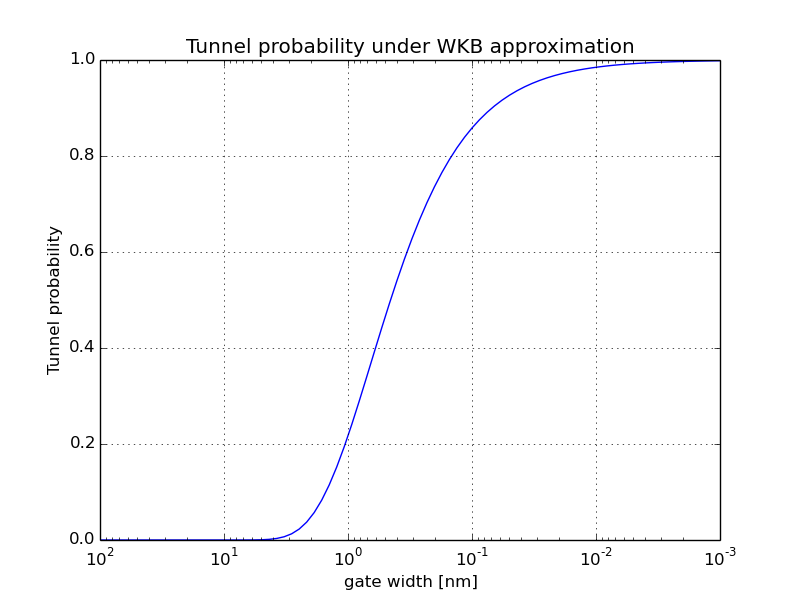
\includegraphics[width=0.6\textwidth]{wkb}
 

\end{itemize}
\end{overprint}


\end{frame}


\begin{frame}\frametitle{Possible candidates?}
  \begin{itemize}
  \pause
   \item Tunnel FETS
   \item Gallium-Arsenide transistors
   \item Mott insulators
   \item Organic semiconductors
   \item Graphene transistors
   \item Photoemission-based microelectronic devices
   \item etc.
  \end{itemize}

\end{frame}

\subsection{Tunnel FET (TFET)}
\begin{frame}\frametitle{Tunnel Field Effect Transistor (TFET)} 
\begin{columns}
\begin{column}{5.8cm}
\begin{overprint}
\onslide<1>
\begin{itemize}
\item Idea: use quantum tunneling!
\item \textit{p-i} and \textit{i-n} junctions are used
\end{itemize}

\onslide<2>
\begin{itemize}
\item In Off-state, all charge carriers are initially in the valence band 
\item In On-state, the energy level of the intrinsic area is lowered with gate-voltage, which leads to a narrowing of the tunnel wall.
\item The electrons tunnel from valence band to conducting band $\rightarrow$ current!
\end{itemize}
\end{overprint}

\end{column}
\begin{column}{6cm}
\begin{center}
\begin{overprint}

\only<1>{\includegraphics[width=0.9\textwidth]{tfet_architecture}}
%\only<2>{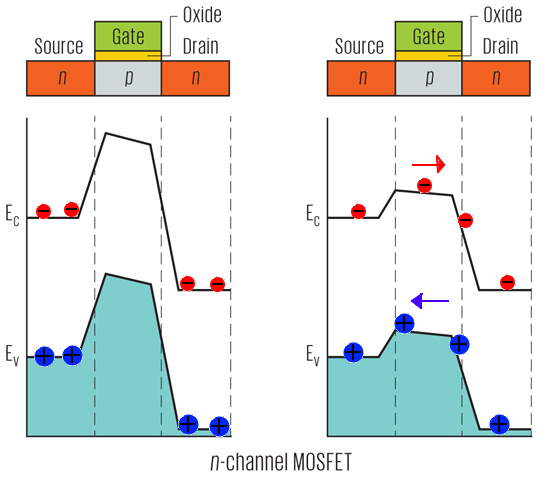
\includegraphics[width=0.9\textwidth]{MOSFETvs}}
\only<2>{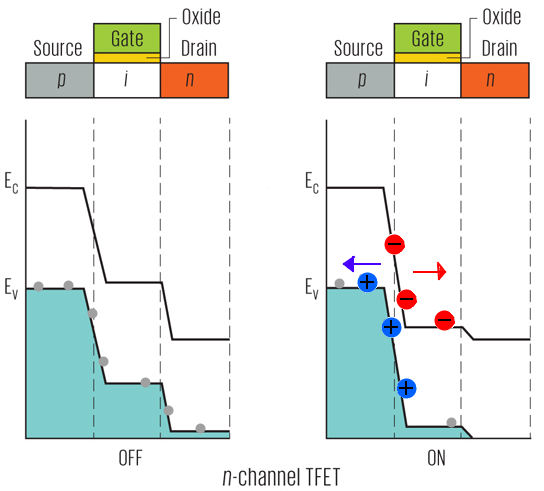
\includegraphics[width=0.9\textwidth]{TFET}}

\only<2>{\mbox{\structure{\tiny{Figure:}}\tiny{ \url{http://spectrum.ieee.org/semiconductors}}}}

\end{overprint}
\end{center}
\end{column}
\end{columns}
\end{frame}

\begin{frame}\frametitle{Advantages and disadvantages of TFETs}
\begin{columns}
\begin{column}{5.8cm}
\begin{itemize}
  \item<1-> Much lower barrier thickness necessary ($\sim$ 1 atom) \newline $\rightarrow$ size could be drastically reduced
  \item<2-> Theoretically not limited by the MOSFETs drain current subthresholdswing limit of 60mV/dec
  \item<3-> Team at IBM created a nanotube based TFET with SS of around 40mV/dec
\end{itemize}
\end{column}
\begin{column}{6cm}
\begin{overprint}

\only<3->{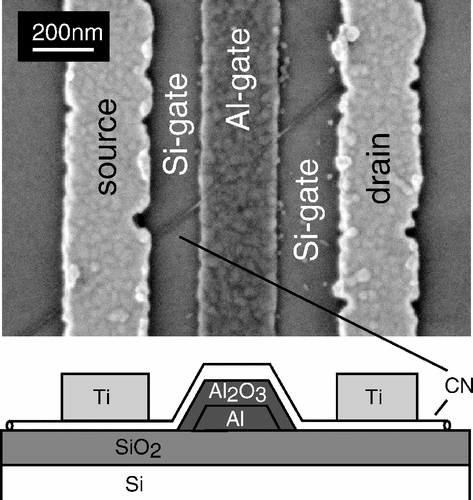
\includegraphics[width=0.7\textwidth]{tfet_jorg}}

\only<3->{\mbox{\structure{\tiny{Figure:}}\tiny{ \url{Appenzeller, J.(2004). Physical Review Letters 93 (19)}}}}



%\only<2>{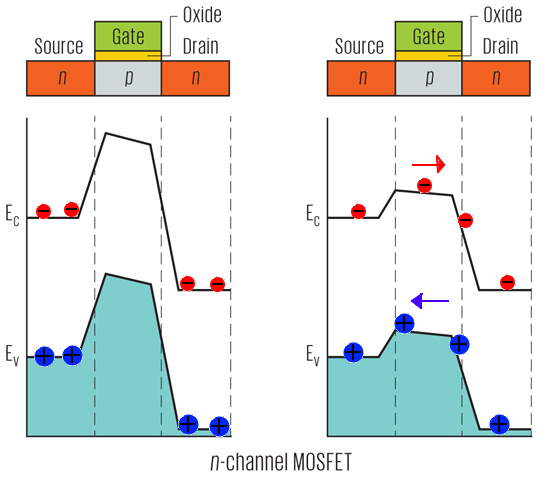
\includegraphics[width=0.9\textwidth]{MOSFETvs}}
%\only<2>{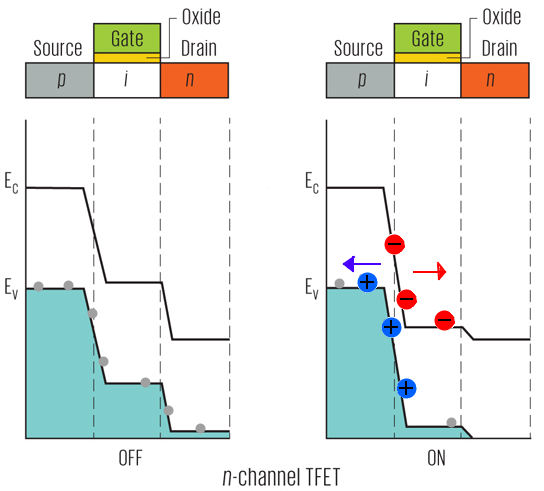
\includegraphics[width=0.9\textwidth]{TFET}}

%\only<1>{\mbox{\structure{\tiny{Figure:}}\tiny{ \url{http://spectrum.ieee.org/semiconductors}}}}

\end{overprint}
\end{column}
\end{columns}
\end{frame}

\begin{frame}
 \begin{itemize}
  \item For quantum tunneling purposes it is better to use direct-band-gap materials, where silicon has an indirect band gap. Manufacturing processes would have to be changed completely. \pause
  \item By using different materials, the chances also rises that the electrons just tunnel straight from source to drain \pause
  \item No devices (processors) yet that use TFET's.
 \end{itemize}
\end{frame}


\section{Sources}
\begin{frame}\frametitle{Sources}
\begin{itemize}
\begin{tiny}
 \item U. Tietze \& Ch. Schenk, Halbleiter-Schaltungstechnik (Springer, Heidelberg, 2010)
 \item S.M. Sze, Semiconductor Devices (Wiley, New York, 1985)
 \item B. El-Kareh, Silicon Devices and Process Integration (Springer, New York, 2009)
 \item Ch. Kittel, Solid State Physics (Wiley, New York, 1999)
 \item U. Straumann, Elektronik fur Physiker (UZH, Zürich, 2005)
 \item \url{https://www.westfloridacomponents.com/blog/transistors}
 \item \url{http://www.electronics-tutorials.ws/transistor/tran_6.html}
 \item \url{http://www.vacuumtubes.net/How_Vacuum_Tubes_Work.htm}
 \item \url{http://spectrum.ieee.org/semiconductors}
 \item J. Appenzeller, Y.-M. Lin, J. Knoch, Band-to-Band Tunneling in Carbon Nanotube Field-Effect Transistors (IBM, New York, 2004)
 \item E. Forati, E. et al. Photoemission-based microelectronic devices. (Nature  Commun. 7, New York, 2016)
\end{tiny}
\end{itemize}
\end{frame}


\section{Questions}
\begin{frame}
\begin{center}
\begin{large}

Questions?
\end{large}
\end{center}
\end{frame}


\section{Backup Slides}
\begin{frame}
\begin{center}
\begin{large}

Backup Slides
\end{large}
\end{center}
\end{frame}

\begin{frame}\frametitle{Bipolar Junction Transistor (BJT)} 
\begin{columns}
\begin{column}{6cm}
\begin{itemize}
\item Combination of two junction diodes (\textit{n-p-n} or \textit{p-n-p}) \newline

\item Emitter, Base, Collector \newline

\item emitter-collector-current is controlled by current on base. \newline

\item EB in forward-bias, CE in reverse-bias

\end{itemize}
%\vspace{3cm} 
\end{column}
\begin{column}{5cm}
%\begin{overprint}
\begin{figure}[H]
\centering
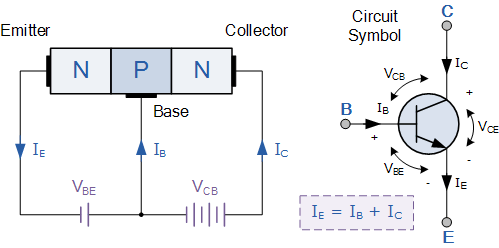
\includegraphics[width=1.1\textwidth]{npn}
\caption{\url{http://www.electronics-tutorials.ws}}%
%\label{fig:npn}
\end{figure}
%\end{overprint}
\end{column}
\end{columns}
\end{frame}

\begin{frame}\frametitle{Bipolar Junction Transistor (BJT)} 
\begin{columns}
\begin{column}{6cm}
\begin{itemize}
\item \textit{Cut-Off Region}: $I_B=0$ $\rightarrow$ no CE-current. 

\item \textit{Saturation Region}: $I_B>0$ and $V_{CE}$ small $\rightarrow$ large CE-current, no control 

\item \textit{Active Region}: $I_B>0$ and $V_{CE}$ large $\rightarrow$ CE-current controlled by base-current

\end{itemize}
%\vspace{3cm} 
\end{column}
\begin{column}{5cm}
%\begin{overprint}
\begin{figure}[H]
\centering
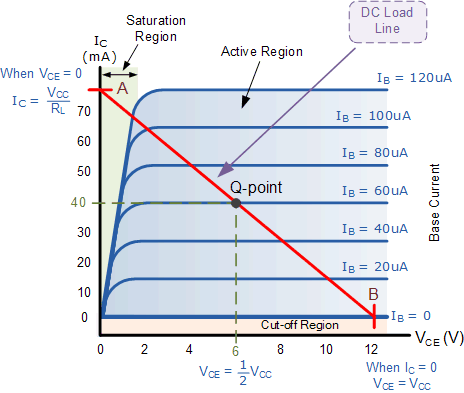
\includegraphics[width=1.1\textwidth]{kenn_npn}
\caption{\url{http://www.electronics-tutorials.ws}}%
%\label{fig:kenn_npn}
\end{figure}
%\end{overprint}
\end{column}
\end{columns}
\end{frame}

%\begin{frame}\frametitle{Logic Gates}
%\begin{columns}
%\begin{center}
%\begin{large}
%AND
%\end{large}
%\end{center}
%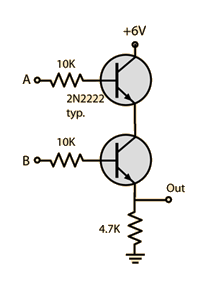
\includegraphics[width=0.6\textwidth]{and}
%\caption{\url{http://hyperphysics.phy-astr.gsu.edu}}%
%\end{column}
%\begin{column}{5cm}
%\begin{center}
%\begin{large}
%OR
%\end{large}
%\end{center}
%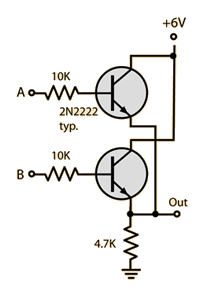
\includegraphics[width=0.6\textwidth]{or}
%\caption{\url{http://hyperphysics.phy-astr.gsu.edu}}%
%\end{column}
%\end{columns}
%\end{frame}




\begin{frame}\frametitle{Manufacturing Process} 
\begin{overprint}
 \begin{enumerate}
  \item Create Wafer: Sand $\xrightarrow{melting}$ Monochrystalline Silicon Ingot $\xrightarrow{slicing}$ Silicon Wafer
  \item Photolithography: Applying photoresist chemical to Wafer $\rightarrow$ Exposure by masked UV-rays $\rightarrow$ Removal of soluble photoresist chemicals
  \item Doping: Patterned photoresist is exposed by a beam of ions (n-type \& p-type) $\rightarrow$ Removal of photoresist chemicals
  \item Etching: Protect desired parts by hard mask $\rightarrow$ Photolithography again
  \item Gate Formation: Form temporarily gate with silicon $\rightarrow$ Fill areas with insulator $\rightarrow$ Add dielectric $\rightarrow$ Electroplating
 \end{enumerate}
\end{overprint}
\end{frame}

\begin{frame}\frametitle{Logic Gates}
 \begin{overprint}
 \begin{center}
  \only<1>{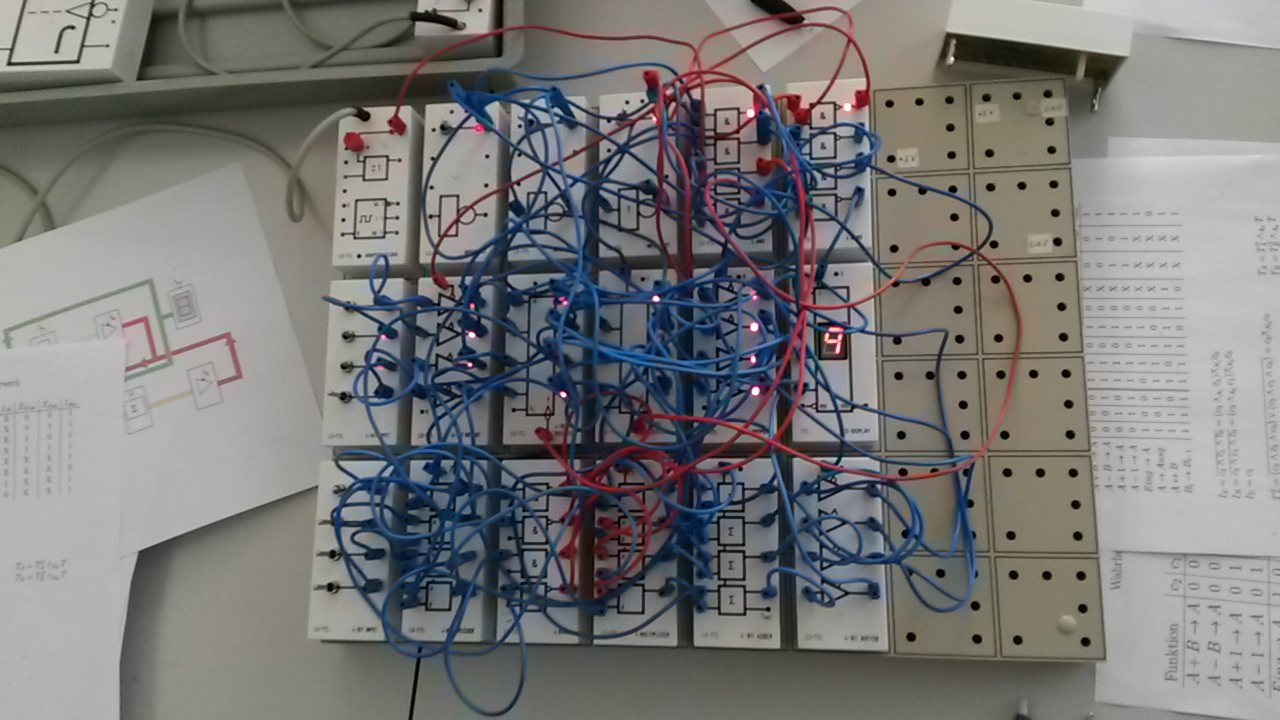
\includegraphics[width=0.8\textwidth]{9.jpg}}
  \only<2>{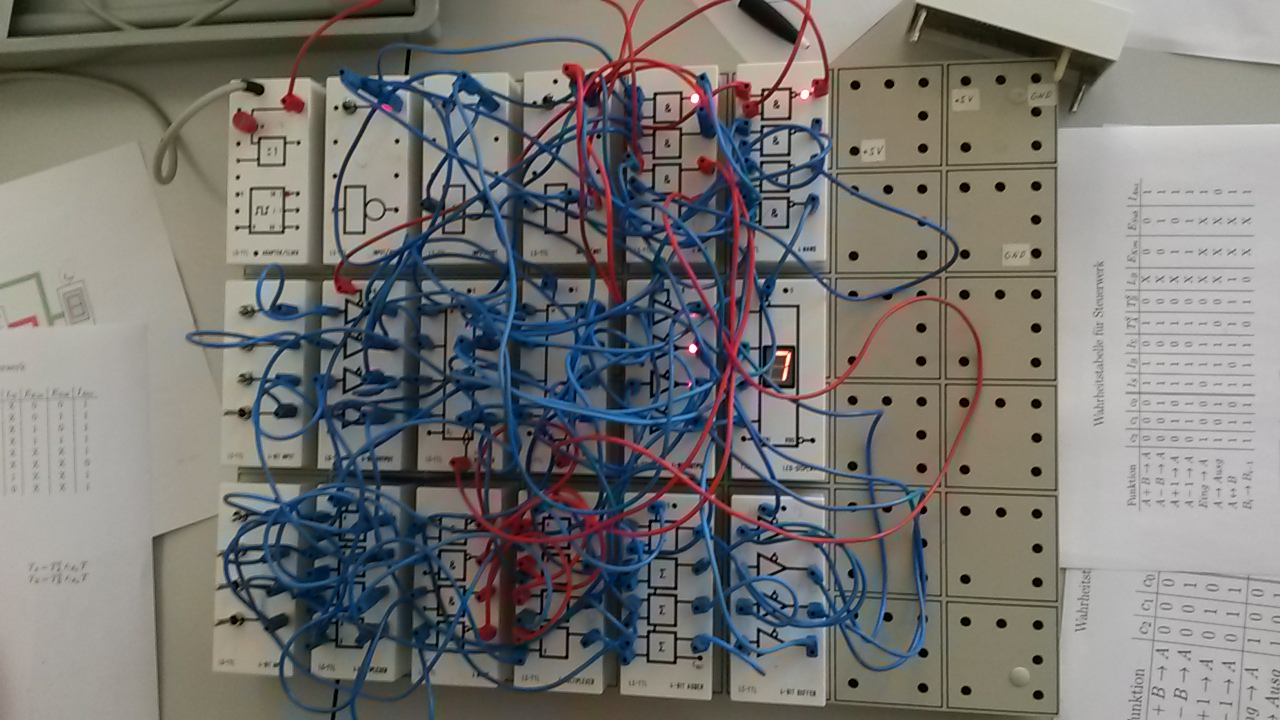
\includegraphics[width=0.8\textwidth]{7}}
  \only<3>{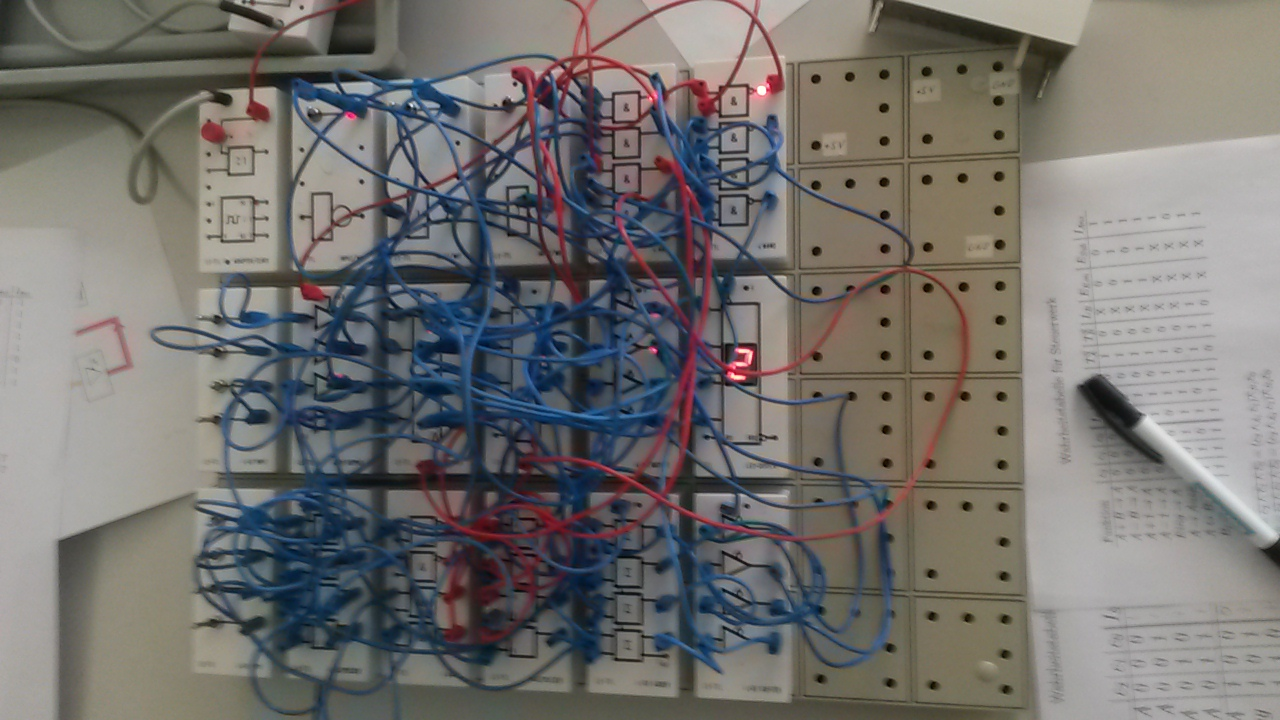
\includegraphics[width=0.8\textwidth]{2}}  
  \only<4>{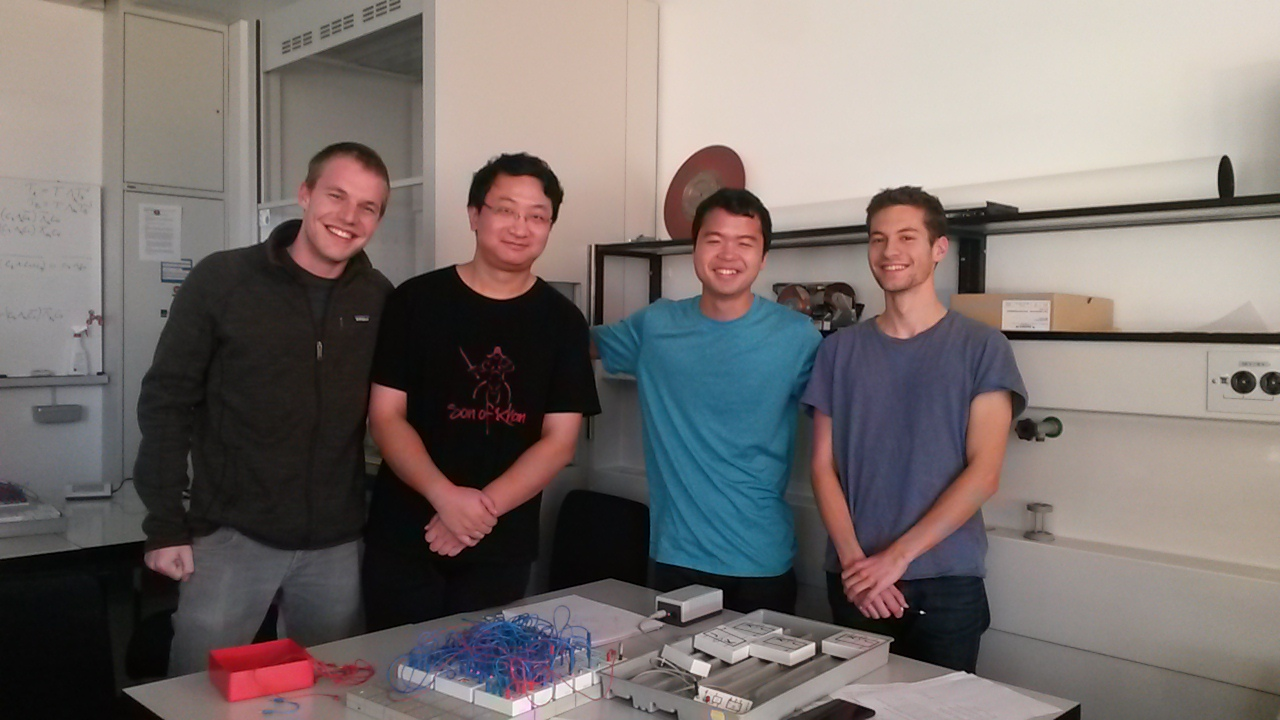
\includegraphics[width=0.8\textwidth]{victory}}  
 \end{center}
 \end{overprint}

\end{frame}



\end{document}